\chapter{Weryfikacja poprawności działania systemu}


(Tutaj stworzyłbym tabelę z adresami ip i zweryfikował czy każde z urządzeń może się komunikować z sąsiadem. Dodatkowo zawarłbym jakiś zrzut ekranu z tablicy rutingu, tablicy dzieci ruterów. Kolejne omówię przebiegi czasowe na rysunkach i opiszę, czy zgadzają się z założeniami, poprzednio przytoczywszy parę podstawowych informacji o grafanie)

    \begin{figure}[H]
        \centering
        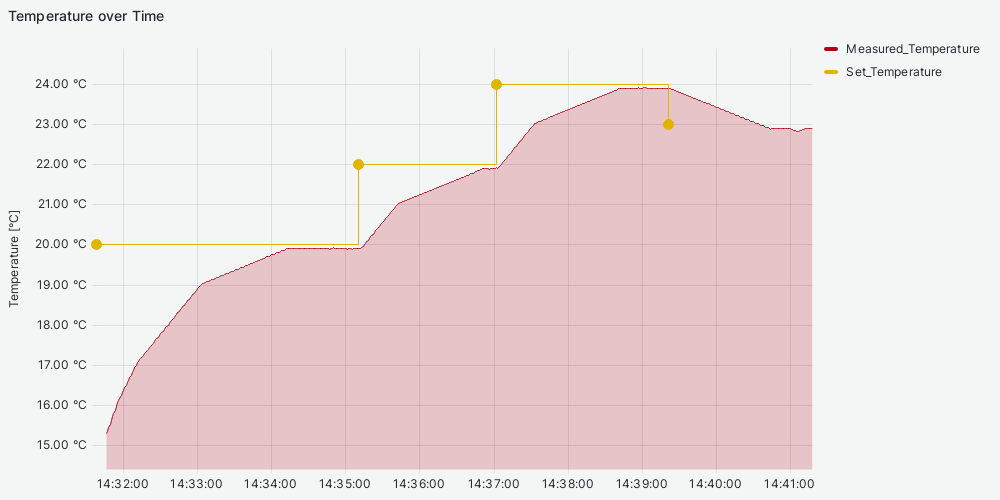
\includegraphics[width=0.8\linewidth]{graphics/grafana/temperature-lm.png}
        \caption{Przebiegi czasowe zmierzonej oraz ustalonej temperatury.}
        \label{fig:graph-heater-temperature}
    \end{figure}

    \begin{figure}[H]
        \centering
        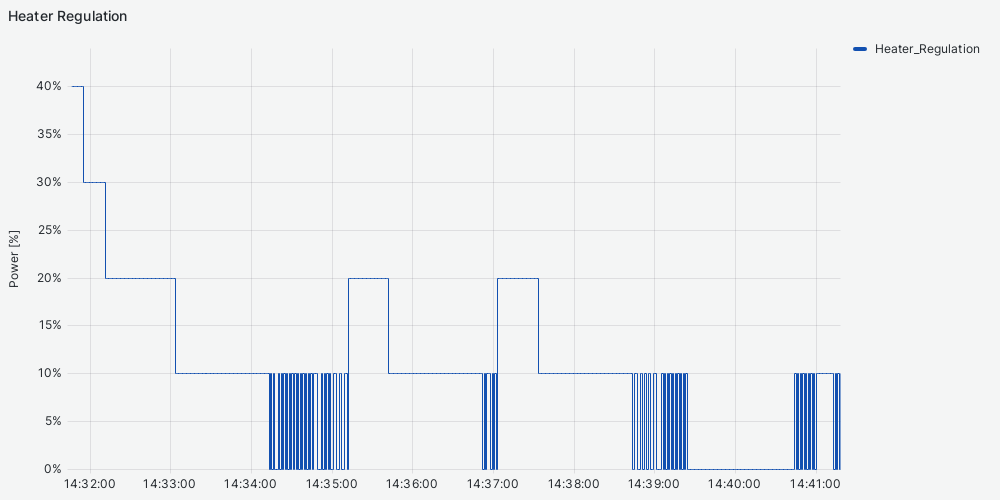
\includegraphics[width=0.8\linewidth]{graphics/grafana/heater-regulation-lm.png}
        \caption{Przebieg czasowy regulacji mocy układu HEATER.}
        \label{fig:graph-heater-regulation}
    \end{figure}

    \begin{figure}[H]
        \centering
        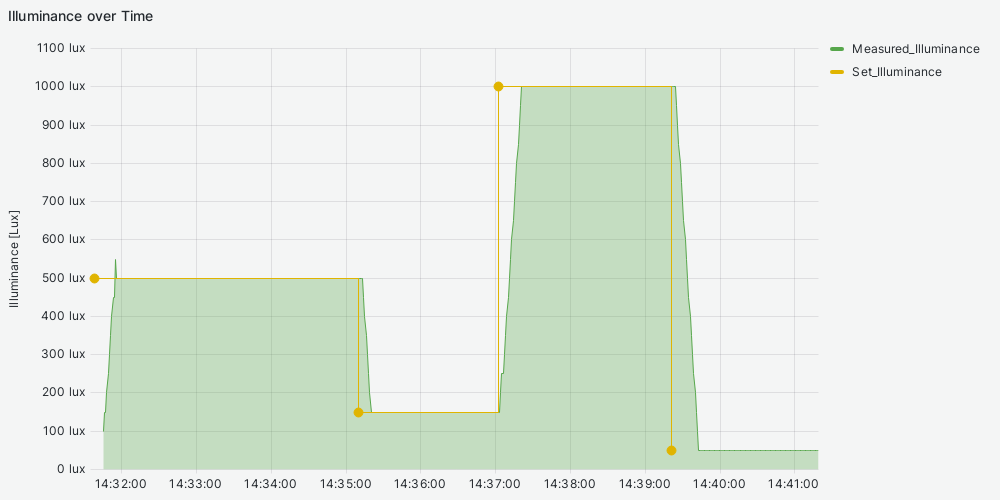
\includegraphics[width=0.8\linewidth]{graphics/grafana/illuminance-lm.png}
        \caption{Przebiegi czasowe zmierzonego oraz ustalonego natężenia oświetlenia.}
        \label{fig:graph-dimmer-illuminance}
    \end{figure}

    \begin{figure}[H]
        \centering
        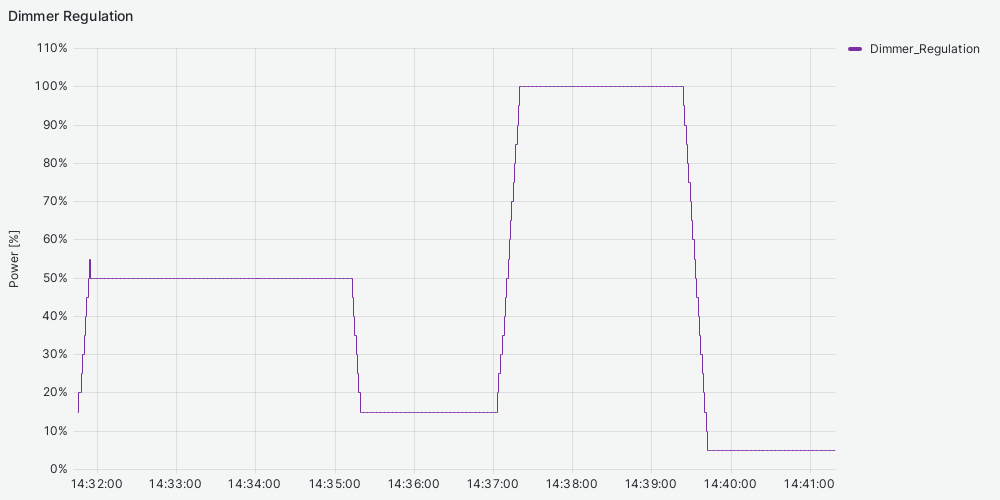
\includegraphics[width=0.8\linewidth]{graphics/grafana/dimmer_regulation-lm.png}
        \caption{Przebieg czasowy regulacji mocy układu DIMMER.}
        \label{fig:graph-dimmer-regulation}
    \end{figure}